\newpage

\section[Day 15: Continuity Properties]{Properties of Continuity}

\subsection{ Continuity and Compactness }

{ \color{blue} Definition 15.1.1: Bounded Functions }

    \begin{adjustbox}{minipage=14cm, right, vspace=0.1cm 0cm}
        f: E $\rightarrow$ $\mathbb{R}^k$ is bounded if there is a
        M $\in$ $\mathbb{R}$ such that f(x) $\leq$ M for all x $\in$ E.
    \end{adjustbox}

    \vspace{0.5cm}

{ \color{red} Theorem 15.1.2:
Continuous functions from compact spaces are compact }

    \begin{adjustbox}{minipage=14cm, right, vspace=0.1cm 0cm}
        Suppose f is a continuous mapping of a compact metric space X
        into a metric space Y. Then f(X) is compact.
    \end{adjustbox}

{ \color{magenta} \underline{Proof} }

    \fbox{
    \begin{minipage}{15cm}
        Let \{$V_{\alpha}$\} be an open cover of f(X).
        Since f is continuous, then by {\color{red} theorem 14.2.4},
        each $f^{-1}(V_{\alpha})$ is open.

        Since X is compact, there is a n such that
        X $\subset$ $f^{-1}(V_{\alpha_1})$ $\cup$ ... $\cup$ $f^{-1}(V_{\alpha_n})$.

        Thus, f(X) $\subset$ $V_{\alpha_1}$ $\cup$ ... $\cup$ $V_{\alpha_n}$
        so f(X) is compact.
    \end{minipage} }

\begin{figure}[h]
    \centering
	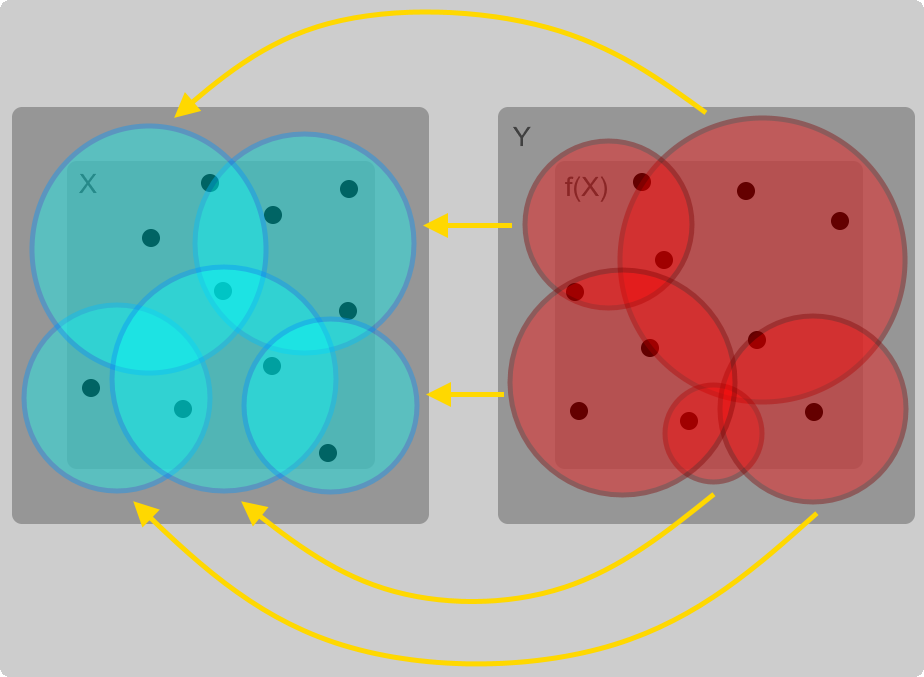
\includegraphics[scale=0.28]{Images/15.1.2.png}
\end{figure}

{ \color{red} Theorem 15.1.3:
Continuous functions from compact to $\mathbb{R}^k$ are bounded }

    \begin{adjustbox}{minipage=14cm, right, vspace=0.1cm 0cm}
        If f is a continuous mapping of a compact metric space X into $\mathbb{R}^k$,
        then f(X) is closed and bounded. 
    \end{adjustbox}

{ \color{magenta} \underline{Proof} }

    \fbox{
    \begin{minipage}{15cm}
        By {\color{red} theorem 15.1.2}, f(X) is compact.
        
        Then by {\color{red} theorem 8.3.13}, f(X) is closed and bounded.
    \end{minipage} }

    \vspace{0.5cm}

{ \color{red} Theorem 15.1.4: Generalized extreme value theorem }

    \begin{adjustbox}{minipage=14cm, right, vspace=0.1cm 0cm}
        Suppose f is a continuous real function of a compact metric space X
        such that M = sup$_{x \in X}$ f(x) and m = inf$_{x \in X}$ f(x).

        Then there exists p,q $\in$ X such that f(p) = M and f(q) = m.
    \end{adjustbox}

{ \color{magenta} \underline{Proof} }

    \fbox{
    \begin{minipage}{15cm}
        By {\color{red} theorem 15.1.3}, f(X) is closed and bounded.
        
        Let M = sup$_{x \in X}$ f(x) and m = inf$_{x \in X}$ f(x).

        Since f(X) is bounded, then M,m $\in$ (f(X))' and
        since f(X) is closed, then M,m $\in$ f(X).
        Thus, there exists p,q $\in$ X such that f(p) = M and f(q) = m.
    \end{minipage} }

\newpage

{ \color{red} Theorem 15.1.5: If f is continuous 1-1, then $f^{-1}$ is continuous }

    \begin{adjustbox}{minipage=14cm, right, vspace=0.1cm 0cm}
        Suppose f is a continuous 1-1 mapping of a compact metric space X
        onto a metric space Y.
        Then $f^{-1}$ is a continuous mapping of Y onto X.
    \end{adjustbox}

{ \color{magenta} \underline{Proof} }

    \fbox{
    \begin{minipage}{15cm}
        Let V be an open set in X.

        Since $V^c$ is closed and $V^c$ $\subset$ compact set X,
        then by {\color{red} theorem 8.3.5}, $V^c$ is compact.

        Thus by {\color{red} theorem 15.1.2}, f($V^c$) is a compact
        subset of Y so f($V^c$) is closed.

        Since f is 1-1 and onto, f($V^c$) = $(f(V))^c$ so f(V) is open.
        Since from any open set V in X, f(V) is open in Y, then by
        {\color{red} theorem 14.2.4}, $f^{-1}$ is continuous.
    \end{minipage} }

    \vspace{0.5cm}

{ \color{blue} Definition 15.1.6: Uniformly Continuous }

    \begin{adjustbox}{minipage=14cm, right, vspace=0.1cm 0cm}
        Let f: X $\rightarrow$ Y. Then f is uniformly continuous on X if:
        
        \begin{adjustbox}{minipage=13cm, right, vspace=0.1cm 0cm}
            For every $\epsilon > 0$, there is a $\delta > 0$
            such that for all p,q $\in$ X
            
            where $d_X(p,q) < \delta$, then
            $d_Y(f(p),f(q)) < \epsilon$.
        \end{adjustbox}
    \end{adjustbox}

    \vspace{0.5cm}

{ \color{red} Theorem 15.1.7:
Continuous functions from compact are uniformly continuous }

    \begin{adjustbox}{minipage=14cm, right, vspace=0.1cm 0cm}
        Let f be a continuous mapping of a compact metric space X into
        metric space Y.
        Then f is uniformly continuous on X.
    \end{adjustbox}

{ \color{magenta} \underline{Proof} }

    \fbox{
    \begin{minipage}{15cm}
        For $\epsilon > 0$, since f is continuous, then for each
        p $\in$ X, there is a $\phi(p)$ such that for all q $\in$ X
        where $d_X(q,p) < \phi(p)$, $d_Y(f(q),f(p)) < \frac{\epsilon}{2}$.

        Let J(p) be the set of all q $\in$ X where
        $d_X(q,p) < \frac{1}{2}\phi(p)$.

        Since the set of all J(p) is an open cover of X and since X is compact,
        then there is a n such that X $\subset$ J($p_1$) $\cup$ ... $\cup$ J($p_n$).
        Let $\delta$ = $\frac{1}{2}$ min( $\phi(p_1), ... , \phi(p_n)$ ) $>$ 0.

        Then for p,q $\in$ X where $d_X(p,q) < \delta$, there is a m where
        $1 \leq m \leq n$ such that p $\in$ J($p_m$) so
        $d_X(p,p_m) < \frac{1}{2} \phi(p_m)$. Thus:

        \hspace{1cm}
        $d_X(q,p_m) \leq d_X(q,p) + d_X(p,p_m) < \delta + \frac{1}{2} \phi(p_m)
        \leq \phi(p_m)$

        \hspace{1cm}
        $d_Y(f(p),f(q)) \leq d_Y(f(p),f(p_m)) + d_Y(f(p_m),f(q))
        < \frac{\epsilon}{2} + \frac{\epsilon}{2} = \epsilon$
    \end{minipage} }

    \vspace{0.5cm}

{ \color{red} Theorem 15.1.8:
Continuous functions from noncompact $\not \rightarrow$ uniformly continuous }

    \hspace{1cm}
    Let E be a noncompact set in $\mathbb{R}^1$.

    \begin{enumerate}[label=(\alph*), leftmargin=2cm, itemsep=0.1cm]
        \item There exists a continuous function which is not bounded.
        
        \item There exists a continuous, bounded function which is
        has no maximum.
        
        \item If E is bounded, there exists a continuous function which
        is not uniformly continuous.
    \end{enumerate}

{ \color{magenta} \underline{Proof} }

    \fbox{
    \begin{minipage}{15cm}
        Suppose E is bounded so there is a $x_0$ $\in$ E', but $x_0$ $\not \in$ E.

        Consider f(x) = $\frac{1}{x - x_0}$ which is continuous on E, but unbounded.

        For $\epsilon > 0$ and $\delta > 0$, there is a x $\in$ E such that
        $|x - x_0| < \delta$.
        Take t close enough to $x_0$ so $|f(t) - f(x_0)| > \epsilon$,
        but $|t - x| < \delta$.
        Thus, f is not uniformly continuous.

        \vspace{0.2cm}

        Consider g(x) = $\frac{1}{1 + (x - x_0)^2}$ which is continuous on E
        and bounded since g(x) $\in$ (0,1).

        Since sup$_{x \in E}$ g(x) = 1, but g(x) $<$ 1 for all x $\in$ E, then
        g has no maximum on E.
    \end{minipage} }

    \newpage





\subsection{ Continuity and Connectedness }

{ \color{red} Theorem 15.2.1: Continuous functions map connected to connected }

    \begin{adjustbox}{minipage=14cm, right, vspace=0.1cm 0cm}
        If f is a continuous mapping of X into Y and E is a connected
        subset of X, then f(E) is connected.
    \end{adjustbox}

{ \color{magenta} \underline{Proof} }

    \fbox{
    \begin{minipage}{15cm}
        Suppose f(E) = A $\cup$ B where A and B are nonempty separated
        subsets of Y.
        
        Let G = E $\cap$ $f^{-1}(A)$ and H = E $\cap$ $f^{-1}(B)$.
        Then E = G $\cup$ H.

        Since A $\subset$ $\overline{A}$, G $\subset$ $f^{-1}(\overline{A})$.
        Since f is continuous, then $f^{-1}(\overline{A})$ is closed so
        $\overline{G}$ $\subset$ $f^{-1}(\overline{A})$.
        Thus, f($\overline{G}$) $\subset$ $\overline{A}$.

        Since f(H) = B and $\overline{A}$ $\cap$ B is empty,
        $\overline{G}$ $\cap$ H is empty.
        Similarily, G $\cap$ $\overline{H}$ is empty so G and H are separated
        which contradicts that E = G $\cup$ H is connected.
    \end{minipage} }

    \vspace{0.5cm}

{ \color{red} Theorem 15.2.2: Generalized Intermediate Value Theorem }

    \begin{adjustbox}{minipage=14cm, right, vspace=0.1cm 0cm}
        Let f be a continuous real function on [a,b]. If f(a) $<$ c $<$ f(b),
        then there exists x $\in$ (a,b) such that f(x) = c.
    \end{adjustbox}

{ \color{magenta} \underline{Proof} }

    \fbox{
    \begin{minipage}{15cm}
        Since [a,b] is connected, then by {\color{red} theorem 15.2.1},
        f([a,b]) is a connected subset of $\mathbb{R}^1$.

        Thus, by {\color{red} theorem 9.2.2}, any c where f(a) $<$ c $<$ f(b)
        is c $\in$ f(x) for some x $\in$ [a,b].
    \end{minipage} }

    \vspace{0.5cm}







